%% Template for a preprint Letter or Article for submission
%% to the journal Nature.
%% Written by Peter Czoschke, 26 February 2004
%%

\documentclass[12pt,twocolumn]{article}

\usepackage{times}
\usepackage{graphicx}
\usepackage[swedish]{babel}
\usepackage[utf8]{inputenc}


\renewcommand{\baselinestretch}{1.5} 
\newenvironment{affiliations}{%
    \setcounter{enumi}{1}%
    \setlength{\parindent}{0in}%
    \slshape\sloppy%
    \begin{list}{\upshape$^{\arabic{enumi}}$}{%
        \usecounter{enumi}%
        \setlength{\leftmargin}{0in}%
        \setlength{\topsep}{0in}%
        \setlength{\labelsep}{0in}%
        \setlength{\labelwidth}{0in}%
        \setlength{\listparindent}{0in}%
        \setlength{\itemsep}{0ex}%
        \setlength{\parsep}{0in}%
        }
    }{\end{list}\par\vspace{12pt}}

%% Redefine the abstract environment to be the first bold paragraph
\renewenvironment{abstract}{%
    \setlength{\parindent}{0in}%
    \setlength{\parskip}{0in}%
    \bfseries%
    }{\par\vspace{-6pt}}

%% Define the addendum environment for Supplementary Info, Acknowledgements, etc.
\newenvironment{addendum}{%
    \setlength{\parindent}{0in}%
    \small%
    \begin{list}{Acknowledgements}{%
        \setlength{\leftmargin}{0in}%
        \setlength{\listparindent}{0in}%
        \setlength{\labelsep}{0em}%
        \setlength{\labelwidth}{0in}%
        \setlength{\itemsep}{12pt}%
        \let\makelabel\addendumlabel}
    }
    {\end{list}\normalsize}

\newcommand*{\addendumlabel}[1]{\textbf{#1}\hspace{1em}}



%\documentclass{nature}
%\documentclass{article}


%% make sure you have the nature.cls and naturemag.bst files where
%% LaTeX can find them



\bibliographystyle{naturemag}

\title{Det är bara ett litet stick i fingret}

%% Notice placement of commas and superscripts and use of &
%% in the author list

\author{Geraldine Lang$^{1}$, Liv Lomax$^1$, Stefan Lang$^3$,Lennart
Johansson$^2$}


\begin{document}

\onecolumn

\maketitle

\begin{affiliations}
 \item ST-läkare i Allmänmedicin, Näsets Läkargrupp
 \item Specialist läkare i Allmänmedicin, Näsets Läkargrupp
 \item Statistiker vid Divisionen för Molekylär Hematologi, Lund universitet
\end{affiliations}

\begin{abstract}
Abstract is missing up to now!
\end{abstract}


\twocolumn

\newpage

\section{Backgrund}

Would that work now: ``ÜäÖäö''

Rädsla och smärta i samband med provtagning på barn är vanligt
förekommande, men sällan något vi läkare behöver konfronteras med
när vi skickar ut barnet till labbet. Ju mindre barnet är desto svårare
har det att förstå nödvändigheten av en ibland smärtsam procedur och
reagerar med rädsla och oro. Inte bara fysisk skada kan leda till smärta
utan även förväntad smärta kan leda till oro och ångest, som i sin
tur förstärker smärtupplevelsen \cite{Carverius2014}.
Man trodde länge att små barn inte kunde känna smärta på samma
sätt som vuxna då deras nervsystem var omoget \cite{Rey1993}. Under de
senaste 30
åren har forskning kring barns smärta dock visat att att även små
barn har ett minne av smärta \cite{Anand2007,Fitzgerald2001,Schechter2003}.
Minnen av smärtsamma upplevelser kan bidra till negativa upplevelser av
vården och därmed försvåra barnets framtida kontakter med
sjukvården \cite{vBayer2004}. Dessa aspekter ger oss läkare ett stort
ansvar och är något som vi behöver beakta i vår kliniska vardag.

En betydande andel av besök på VC utgörs av små barn med
infektionssymtom. De patientnära analyserna för identifiering av
Betahemolytiska streptokocker grupp A (Strep-A) och C-reaktivt protein (CRP)
är diagnostiska verktyg i läkarens kliniska vardag, som i bästa fall kan
minska läkarens osäkerhet och förbättra diagnossättning vid
infektioner i öppenvården. Men utöver att vara förknippat med smärta
och oro är tolkning av testresultaten inte helt okomplicerat.
Exempelvis ger analys av CRP, ett akutfasprotein som stiger vid
infektionssjukdomar och inflammation, sällan vägledning för om antibiotika
behövs eller ej. Vid okomplicerad infektion utan allmänpåverkan har
testet ringa värde och det ska helst ha gått 24 timmar efter insjuknandet
för att testet skall vara tillförlitligt. Vissa lokala allvarliga
infektioner ger heller inte kraftig stegring av CRP tidigt i förloppet
\cite{Tecken2014}.

även identifiering av streptokocktonsilliter med snabbtestet Strep-A, medför
diagnostiska dilemman. Enligt tillverkarna har testet en sensitivitet på $>$
93\% och en specificitet på $>$ 94\%. Ett problem är dock att en betydande
andel av alla barn är bärare av streptokocker vintertid, utan att vara
sjuka. Då merparten av halsinfektioner är orsakade av virus riskerar
testet, om taget på fel grund, att felklassificera virusinfektioner som
streptokocktonsilliter hos bärare.

Trots att det finns påvisat ett samband mellan hög förskrivning av
antibiotika och hög användning av CRP och Strep-A \cite{Studie2014} har
snabbtesterna fortfarande stor användning i primärvården. I en tidigare
studie från Canada har man belyst barns upplevelser och erfarenheter av
venös provtagning \cite{Fradet1990}. I studien har man bland annat visat ett
samband mellan barns ålder och upplevelser vid provtagning samt visat att
föräldrar väl kan förutsäga barnets väntade reaktion under
provtagning \cite{Fradet1990}. Samma studie har även indikerat att
föräldrars oro korrelerar med barnets stressupplevelse vid venös
provtagning.

Vi känner inte till någon studie som tittat på barn och föräldrars
erfarenheter av provtagning med de patientnära analyserna CRP och Strep-A. Vi
känner inte heller till att liknande studier genomförts i
primärvården.

Syftet med denna studie var att belysa barns smärtupplevelser vid provtagning.
Vi ville även studera eventuellt samband mellan barns smärtupplevelser och
faktorer som ålder, kön, tidigare exponering för provtagning och
föräldrarnas förutsägelse av barnets smärtreaktion.

\section{Vetenskapliga Frågeställningar}

Hur vanligt förekommande är smärta vid patientnära provtagning på
Näsets Läkargrupp (NLG)?
Finns det skillnad i utfall (självskattad smärta) beroende på barnets
ålder, kön, tidigare exponering för provtagning? Vår hypotes var att
barnets smärtupplevelse avtar med stigande ålder.
Finns samband mellan utfall och föräldrarnas förutsägelse av barnets
reaktion, ev stickrädsla hos föräldrarna? Vår hypotes var att
föräldrar kan förutse sitt barns smärtrespons.

\section{Method}

Barn i åldersgruppen 0-17 år, som skickade till labbet på NLG för
patientnära analys (CRP, Strep-A), ingick i studien. även föräldrar till
barnen som deltog ingick i studien. Deltagandet i studien var oberoende av
symtom barnet sökte för och studien inkluderade även barn med
underliggande kronisk sjukdom.

Innan provtagning, ute i väntrummet, presenterades syftet med studien för
föräldern och barnet med hjälp av ett informationsblad. Föräldern fick
fylla i en kort enkät kring vad barnet hade för besvär vid besöket (t ex
feber, halsont, hosta) samt ange huruvida de upplevde att barnets
allmäntillstånd hade försämrats eller ej senaste dygnet. Föräldern
fick även kryssa för om man hade önskemål om att det skulle tas prov i
samband med besöket, om detta var något man förväntade sig. I
enkäten ombads föräldern uppge om barnet tagit någon prov på VC
(stick i fingret, svalgprov) tidigare och om barnet blev ledsen i samband med
förra provtagningen. Föräldern ombads även skatta, enligt en 10 cm
visuell analog skala, hur dom trodde att barnet skulle reagera vid dagens
provtagning.
Ena änden av skalan definierades som lugn, ingen oro andra änden som
mycket ledsen, mycket orolig. Enligt denna skala ombads föräldern även
skatta vad dom själva tycker om att ta prov.

Direkt efter provtagning ombads föräldern, enligt samma skala som ovan,
skatta hur deras barn tedde sig i väntrummet inför provtagning samt barnets
reaktion under själva provtagningen.

Direkt efter provtagningen bad en sköterska på labbet även barnet skatta
sin upplevda smärta i samband med provtagningen. Barn har i forskning uppgett
att dom föredrar smärtskalor med ansikten (facial pain scales, FPS)
framför andra typer av självskattningsinstrument \cite{vBayer2006}. Av denna
anledning valde vi att använda den välkända Wong-Baker FACES Smärtskala
i vår studie (bild 1). Denna skala visar en serie ansikten där änden vid
0 visar ett glatt ansikte ingen smärta och änden vid 10 visar ett
gråtande ansikte värsta tänkbara smärta.


Smärta är alltid subjektiv och det är en utmaning att utvärdera smärta
hos barn.
Inom hälso- och sjukvården är självskattning ett förstahandsval vid
bedömning av smärta. Ansiktsskalor har visat validitet från 4 års
ålder (11, 12). Då barn i åldersgruppen 0-3 år inte är kapabla
till självskattning, har vi inte haft möjlighet att analysera dessa
uppgifter enligt vårt studieupplägg. Barn yngre än 4 år exkluderades
därför från den delen av studien där barnet ombads skatta sin smärta
i samband med provtagning. Av egen erfarenhet, som både läkare och
förälder, tror vi dock att barn i åldersgruppen 0-3 år är extra
vulnerabla vid provtagning. Vi bad därför föräldrar fylla i enkäten
även för barn under 4 år.

Vi valde att inte sätta någon övre åldersgräns för deltagande av
barn, förutsatt att en förälder medföljde vid läkarbesöket och
provtagningen.

Målsättningen var att samla in enkäter under åtminstone en säsong
med hög förekomsts av infektioner hos barn. Vi samlade in totalt 156
enkäter.
Majoriteten av alla enkäter samlades in under perioden november-16 till
april-17.

Enkäterna utformats så att det framgick vilket test, CRP eller Strep-A,
som analyserades. Några gånger (n=6) hade läkaren ordinerat både
CRP och Strep-A. Då fick barnet skatta sin smärtresponsen enligt FRS för
båda proverna separat.

Resultat från studien kommer att beskrivas deskriptivt. För att studera
samband mellan variabler kommer vi att använda analytisk statistik,
preliminärt Chi-två-test som är en metod som har utvecklats för att
analysera data då variabler har ordinalskala.

Projektet var ett internt forskningsarbete enligt vetenskapliga principer.
Ansökan till etiknämnd genomfördes därför ej. Verksamhetschefen gav
sin tillåtelse till att vår enkätbaserade undersökning
genomfördes. Insamlade uppgifter var helt anonyma och det är inte möjligt
att identifiera patienterna eller deras föräldrar genom enkäten.
Deltagandet var helt frivilligt. Studien kommer inte att publiceras offentligt.

\section{Resultat}

\begin{figure}
 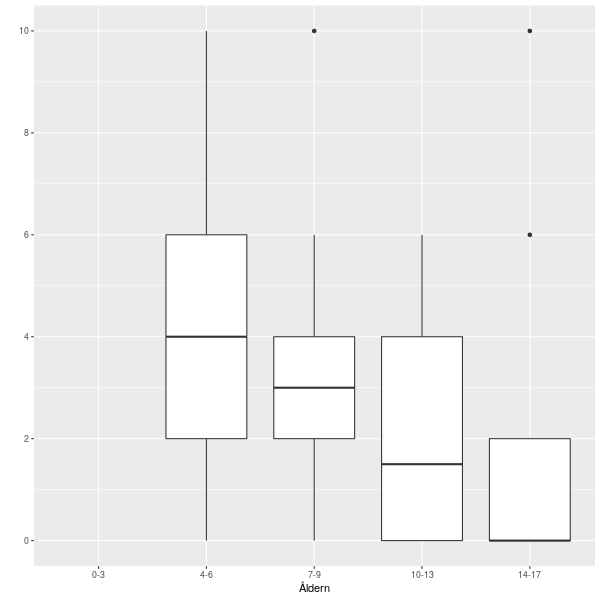
\includegraphics[width=0.5\textwidth]{figures/Question_10_all}
 \caption{ And here we see \ldots }
\end{figure}

\subsection{Studiepopulationen}
Totalt deltog 156 barn och deras föräldrar/närstående i studien. Av
156 barn var 87 flickor och 55 pojkar, medan könet ej hade angivits för 13
deltagare. De yngsta barnen utgjorde den största andelen av vår
studiepopulation. 92 barn (59\%) var $<$ 7 år gamla. För detaljerad
köns- och åldersfördelning se \% tabell 1 och 2.

I 103 enkäter angavs mamma som medföljande, i 39 enkäter angavs pappa. I 4
enkäter angavs att både mamma och pappa var med, medan annan
närstående fyllde i enkäten i 5 fall. I 4 enkäter  saknades
information om medföljande.

133 av 156 barn (85\%) hade tagit prov (CRP och/eller Strep-A) tidigare. Redan i
åldersgruppen 0-3 år hade X\% redan genomgått minst en provtagning
tidigare, se tabell 

Symtom från luftvägarna (hosta, halsont, förkylning, öronvärk
och/eller feber i kombination med något av dessa symtom) utgjorde den
vanligaste besöksorsaken i vår studiepopulation. övriga besöksorsaker
var oklar/isolerad feber, GI-symtom (kräkningar, diarré, magont utan
förkylningssymtom) och UVI symtom. Tabell 3 visar fördelning av
besöksorsaker i populationen.

85\% av alla föräldrar uppgav att dom hade förväntat sig att det skulle
tas \% prov i samband med läkarbesöket. 57\% hade önskemål om detta,
medan 36\% inte \% önskade att det skulle tas något prov (7\% svarade ej
på frågan).

På frågan rörande barnets allmäntillstånd svarade 34\% att
barnets allmäntillstånd hade försämrats senaste dygnet. 50\% uppgav
ett oförändrat allmäntillstånd medan 16\% svarade att barnets
allmäntillstånd hade förbättrats.

Korrelation mellan variabler Vår hypotes var att barnets smärtupplevelse minskar
med stigande ålder. Vår studie visade att ålder är en faktor som korrelerar väl
med hur barnet själv skattar sin smärta vid provtagning för CRP och Strep-A
(diagram xa). Föräldrars observerade också mindre oro och obehag (diagram xb)
med stigande ålder. Deras observation av barnets reaktion under provtagning
korrelerade väl med barnets självskattade smärta (P $<$ 0,001).
Föräldrarna kunde endast kunde fyllde i fråga 9 i enkäten en gång, trots att barnet tog både CRP
och Strep-A, men resultatet var i princip oförändrat när denna lilla grupp barn
(n=6) exkulderades. I den lägsta åldersgrupperna skattade barn i genomsnitt
måttlig smärta (definierat som 4-7 på FPS) vid provtagning för CRP, medan övriga
åldersgrupper endast skattade lindrig smärta (definierat som 0-3 på FPS) vid
provtagning. Vid provtagning Strep-A låg medelvärdet får skattad smärta enligt
FPS på $<$ 4 i samtliga åldersgrupper. Spridningen i självskattad
smärta var, som framgår i diagram x-x stor i flera åldersgrupper.

\section{Diskussion}

Vår studie har visat att en stor andelen av barn som skickas för provtagning på
NLG är yngre än 7 år. Det är oklart om åldersfördelningen i studiepopulationen
speglar åldersfördelningen bland barn som söker med infektionssymtom på NLG då
endast barn som skulle skickas till labbet och deras föräldrar ingick i studien.
En tänkbar möjlighet till åldersfördelningen i studiepopulationen är att läkare
är mer benägna att ta prov på de yngsta barnen. Eventuella förklaringar till
detta vore intressanta att belysa i en framtida studie. Likaså gäller detta
könsfördelningen i studiepopulationen. Det förvånade oss då det generellt var
många fler flickor än pojkar i vår studiepopulation. återigen, är detta
representativt för besökspopulationen eller är läkare mer benägna att ta prov på
flickor? Genom att identifiera de undergrupper av barn som påverkas mest
negativt vid provtagning finns möjlighet att rikta särskild hänsyn till dessa
grupper, såsom extra förberedelse inför provtagning och eventuell intervention
under själva provtagningen (t ex distraktion).

Vår huvudhypotes var att åldern korrelerar med barns smärtupplevelse och att små
barn utgör en undergrupp som behöver ..  Resultat från studien visar att barn i
de yngre åldersgrupperna är mer vulnerabla vid provtagning baserat på deras egen
smärtskattning. Föräldrarnas observation var också att de yngsta barnen tedde
sig mer ledsna och oroliga i samband med provtagning.

Detta är något som vi läkare bör beakta när vi ordinerar prov. I vår studie hade
60.. \% av föräldrarna uppgett att barnets AT var oförändrat eller förbättrat.
Då måste man fråga sig om provtagning, som är något de minsta barnen
förknippar med, verkligen är nödvändig.

I studien framgick också att föräldrar är är bra på att förutse hur deras barn
kommer att reagera i samband med provtagning. Genom att efterhöra hur
föräldrarna tror att deras barn kommer att  reagera finns en möjlighet att fånga
upp de barn som behöver extra stöd och förberedelse. Studien påvisade även ett
samband mellan barnets oro i väntrummet inför provtagningen och smärta och
obehag vid provtagning. Med detta i åtanke tror vi att distraktion/intervention
redan i väntrummet, speciellt riktat mot åldersgrupp 0-9 år, kan minska
stressnivån inför provtagning och därmed barnets obehag vid själva
provtagningen.

\section{Konklusion}

Vi tror att en ökad kunskap kring snabbtesterna kan bidra till färre
slentrianmässigt beställda prover och därigenom ett minskat onödigt lidande för
barnet. Genom att identifiera de eventuella undergrupper av barn som påverkas
mest negativt vid provtagning finns också möjligheter rikta särskild hänsyn till
dessa grupper, såsom extra förberedelse inför provtagning och eventuell
intervention under själva provtagningen (t ex distraktion).




%% Put the bibliography here, most people will use BiBTeX in
%% which case the environment below should be replaced with
%% the \bibliography{} command.
\newpage
\onecolumn

\begin{thebibliography}{1}
\bibitem{Carverius2014} Carverius U, Ljungman G. Smärtbehandling vid procedurer
hos barn- kort historik och dagsläget. Läkemedelsverket, bakgrundsdokumentation 2014;3:24-26. 
\bibitem{Rey1993} Rey R. The history of pain. 1ed. Cambridge, Massachusetts:
Harvard University Press 1993.
\bibitem{Anand2007}Anand K, Stevens B, McGarth PJ. Pain in Neonates and infants:
Pain Research and Clinical Management Series. Elseiver 2007.
\bibitem{Fitzgerald2001}Fitzgerald M, Beggs S. The neurobiology of pain:
developmental aspects. Neuroscientists         2001;7:246-57.
\bibitem{Schechter2003} Schechter N, Berde S, Yaster M. Pain in Infants,
Children, and Adolescents. Lippincott Williams \& Wilkins 2003.
\bibitem{vBayer2004} von Bayer CL, et al. Children memory for pain: overview and implications for practice. J.Pain 2004.
\bibitem{Tecken2014} Tecken på allvarlig infektion hos barn. Ett kunskapsunderlag med förslag till handläggning i primärvård. www.folkhalsomyndigheten.se 2014.
\bibitem{Studie2014} Studie över faktorer som påverkar läkarens beteende vid förskrivning av antibiotika. Resultat från två beteendevetenskapliga studier. www.folkhälsomyndigheten.se 2014.
\bibitem{Fradet1990} Fradet C, McGarth PJ, Kay J, Adams S, Luke B. A prospective survey of reactions to blood        tests by children and adolescents. Pain. Elseiver 1990;40:53-60.
\bibitem{vBayer2006} Von Baeyer C.    Children´s self reports on pain intensity: Scale selection, limitations and            interpretation. Pain Res Management 2006;11:157-162.
\bibitem{Tsze2013} Tsze DS, von Bayer CL, Bullock B, et al. Validation of self-report pain scales in children.     Paediatrics 2013;132:971-9.
\bibitem{WHO2012} WHO. Persisting pain in children Package: Who Guidelines on Pharmacological Treatment   of Persisting Pain in Children with Medical Illnesses. 2012;ISBN 9241548126;30-31.

\end{thebibliography}


%% Here is the endmatter stuff: Supplementary Info, etc.
%% Use \item's to separate, default label is äcknowledgements"


\begin{addendum}
 \item Put acknowledgements here.
 \item[Competing Interests] The authors declare that they have no
competing financial interests.
 \item[Correspondence] Correspondence and requests for materials
should be addressed to A.B.C.~(email: myaddress@nowhere.edu).
\end{addendum}

%%
%% TABLES
%%
%% If there are any tables, put them here.
%%

\end{document}
